\documentclass[UTF8,a4paper,10pt]{ctexart}

\usepackage[top=1.80cm,bottom=1.85cm,left=2.10cm,right=2.10cm]{geometry}
\usepackage{booktabs}
\usepackage{tabularx}
\usepackage{array}
\usepackage{caption}
\usepackage{graphicx}
\usepackage{hyperref}
\usepackage{enumitem}
\usepackage{xcolor}
\usepackage{placeins}

\graphicspath{{figures/}}
\hypersetup{
  colorlinks=true,
  linkcolor=blue!55!black,
  citecolor=blue!55!black,
  urlcolor=blue!55!black
}
\captionsetup{
  font=small,
  labelfont=bf,
  aboveskip=4pt,
  belowskip=0pt
}
\setlength{\parindent}{1em}
\setlength{\parskip}{0pt}
\setlength{\emergencystretch}{2em}
\setlist{nosep,leftmargin=1.6em}
\renewcommand{\arraystretch}{1.12}
\setlength{\textfloatsep}{10pt plus 2pt minus 2pt}
\setlength{\floatsep}{8pt plus 2pt minus 2pt}
\setlength{\intextsep}{8pt plus 2pt minus 2pt}
\renewcommand{\topfraction}{0.90}
\renewcommand{\bottomfraction}{0.80}
\renewcommand{\textfraction}{0.08}
\renewcommand{\floatpagefraction}{0.80}
\ctexset{
  section = {
    beforeskip = 1.6ex plus 0.2ex minus 0.2ex,
    afterskip = 0.7ex plus 0.1ex
  },
  subsection = {
    beforeskip = 1.2ex plus 0.2ex minus 0.2ex,
    afterskip = 0.5ex plus 0.1ex
  }
}
\flushbottom

\newcommand{\pp}{\,\mathrm{pp}}

\title{\textbf{Video Understanding POC 技术研究报告}\\[-0.15em]
\large 人脸质量分桶与超分适用性}
\author{吴止境}
\date{2026年7月}

\begin{document}

\pagestyle{plain}
\maketitle

\begin{abstract}
本报告在冻结的MEVID actor check-in Gallery与316条官方Query协议上，评估人脸质量分桶、CR-FIQA与GFPGAN作为ArcFace前处理的适用性。质量严重程度与产品动作采用双轴定义，FIQA仅作诊断。对预先冻结的40条recoverable Query，原图Rank-1为26/40（65.0\%），GFPGAN为8/40（20.0\%），下降45.0个百分点；配对分析显示救回0条、损害18条。两种纯缩放控制均保持26/40，表明下降来自生成式修复对身份特征的改写，而非尺寸归一化。结果不支持将GFPGAN作为默认身份识别前处理；当前链路应保留原始对齐脸，拒绝unusable和none，并仅将超分用于人工查看或离线诊断。
\end{abstract}

\section{质量分桶与身份保持边界}

\subsection{冻结的双轴分桶逻辑}

质量分桶需要回答两个问题：图像质量有多差，以及产品下一步做什么。当前方案因此保留两个字段：\texttt{rule\_quality}描述质量严重程度，\texttt{eligibility}决定身份识别动作。两者使用相同的尺寸、检测分数、姿态和模糊度观测，但不是一一对应关系。

\begin{table}[!htbp]
\centering
\caption{质量分桶与身份识别动作}
\label{tab:quality-routing}
\small
\begin{tabularx}{\linewidth}{
  >{\raggedright\arraybackslash}p{0.19\linewidth}
  >{\raggedright\arraybackslash}X}
\toprule
\texttt{eligibility} & 判定条件、质量类别与动作\\
\midrule
none & 未检测到可用人脸或无法对齐；quality=none；拒绝。\\
unusable & 分数低于0.5、极端姿态或短边小于20像素；quality=poor；拒绝。\\
recoverable & 通过硬门槛，短边为20--28像素或模糊度落入可恢复区间；quality=marginal或poor；当前身份链路仍用原图。\\
direct & 通过硬门槛且不满足recoverable条件；quality=clear或marginal；原图进入ArcFace。\\
\bottomrule
\end{tabularx}
\end{table}

表\ref{tab:quality-routing}直接给出两轴关系。同一个poor既可能是recoverable，也可能是unusable，因此不能只按质量类别决定产品动作。

\begin{figure}[!htbp]
\centering
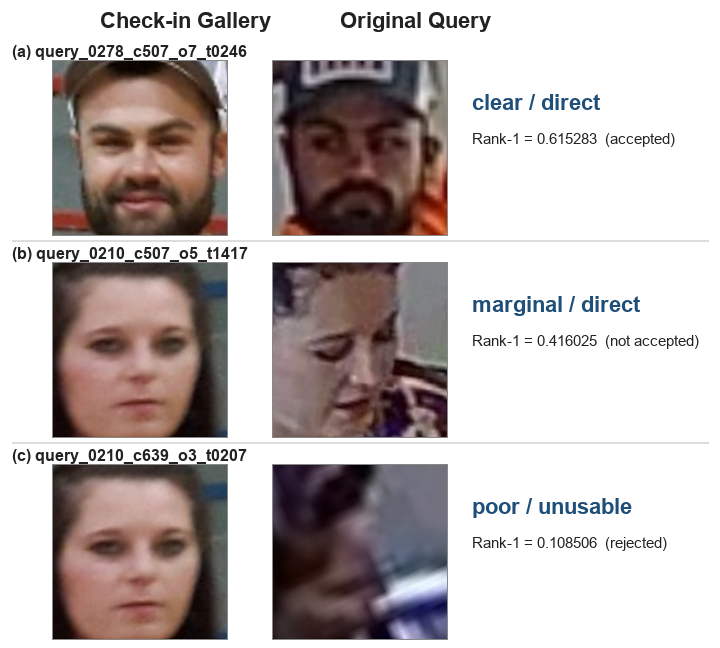
\includegraphics[width=0.72\textwidth]{qualitative_queries.png}
\caption{三个冻结Query样例，按clear、marginal、poor顺序展示真实check-in Gallery与A原图。男性\texttt{query\_0278\_c507\_o7\_t0246}为clear/direct，Rank-1相似度0.615283，产品接受；女性\texttt{query\_0210\_c507\_o5\_t1417}为marginal/direct，Rank-1相似度0.416025，虽第一名身份正确但产品不接受；女性\texttt{query\_0210\_c639\_o3\_t0207}为poor/unusable，Rank-1相似度0.108506，产品拒绝。产品仅在Rank-1相似度$\geq0.45$时接受匹配。}
\label{fig:quality-samples}
\end{figure}

\subsection{为什么CR-FIQA不能保证身份保持}

CR-FIQA用于估计单张人脸是否适合识别\cite{crfiqa}，但它不比较处理前后是否仍为同一身份。生成模型可能把图片变得更清晰，同时改写五官或纹理。此时FIQA可以升高，身份信息却可能下降。

我们在MEVID训练身份上做了单帧诊断。632条候选轨迹中，118条得到有效人脸；最终形成39条参考记录和49条独立测试记录。

\begin{table}[!htbp]
\centering
\caption{CR-FIQA单帧诊断结果}
\label{tab:fiqa}
\small
\begin{tabularx}{0.76\linewidth}{>{\raggedright\arraybackslash}X r}
\toprule
指标 & 结果\\
\midrule
ArcFace第一名正确 & 9/49（18.4\%）\\
第一名正确且达到0.45阈值 & 0/49\\
FIQA与是否认对的相关系数 & 0.026\\
过滤最低10\% FIQA后 & 20.0\%\\
过滤最低20\% FIQA后 & 17.5\%\\
过滤最低50\% FIQA后 & 16.0\%\\
\bottomrule
\end{tabularx}
\end{table}

过滤低FIQA样本没有带来稳定收益。更直接的反例见表\ref{tab:backend-diagnostics}：GFPGAN和CodeFormer提高了FIQA，却显著降低了Rank-1；Real-ESRGAN的FIQA下降，身份结果反而是三个超分后端中最好。FIQA因此不能代替身份保持评估。

\subsection{去掉CR-FIQA后的分桶逻辑}

CR-FIQA现仅保留为诊断字段，不参与建库、质量分桶、超分路由或处理后验收。冻结manifest中的40条recoverable全部由20--28像素尺寸规则确定。关闭FIQA后，这40条的成员完全不变；其中5条虽带有low-FIQA标签，但该标签不是入组原因。后续实验和产品路由均按表\ref{tab:quality-routing}执行。

\section{超分适用性研究}

\paragraph{统一实验设置。}
实验使用MEVID actor check-in正面照建立固定ArcFace Gallery\cite{arcface}：343张合格人脸形成145个身份模板。316条官方Query轨迹各确定性抽取24帧，再在不读取身份结果的前提下选择唯一face-best。最终得到34条direct、40条recoverable、82条unusable和160条none；其中156条可检测并对齐。

所有组共享同一Gallery、Query face-best、ArcFace和0.45接受阈值；产品仅在Rank-1相似度大于等于0.45时接受匹配。GFPGAN与CodeFormer输出512$\times$512，Real-ESRGAN输出224$\times$224；进入ArcFace前均转换为RGB uint8并用LANCZOS归一化为112$\times$112。输入、配置、权重和缓存均被冻结并保存校验值。

\begin{table}[!htbp]
\centering
\caption{固定A/B/C实验组}
\label{tab:protocol}
\small
\begin{tabularx}{\linewidth}{
  >{\centering\arraybackslash}p{0.21\linewidth}
  >{\raggedright\arraybackslash}X}
\toprule
组别 & 处理方式\\
\midrule
A：原图 &
156张可对齐Query全部用原图；仅作诊断对照。\\
B1/B2/B3 &
156张Query分别经过GFPGAN、CodeFormer（$w=1$）和Real-ESRGAN；失败不回退A。\\
C1/C2/C3 &
direct复用A，recoverable复用对应B，unusable和none拒绝；不读取FIQA或识别结果。\\
\bottomrule
\end{tabularx}
\end{table}

两种缩放控制不属于超分后端，只用于排除归一化影响，因此只在GFPGAN实验结果中报告。

\subsection{GFPGAN：原方案为何不适合}

\paragraph{理论判断。}
GFPGAN使用生成式人脸先验补充缺失细节\cite{gfpgan}。这能改善观感，但对身份识别有三个风险。

\begin{enumerate}[label=\arabic*.]
  \item \textbf{合理细节不等于真实细节。} 输入缺少眼睛、轮廓或皮肤信息时，模型只能生成最可能的样子，无法知道真实细节。训练中的身份损失只能降低风险，不能保证身份不变。
  \item \textbf{像素太少时没有唯一答案。} 十几或二十多个像素的人脸没有记录足够的五官信息。PULSE证明，同一低清输入可以对应多张外观不同但都合理的高清人脸\cite{pulse}。
  \item \textbf{去噪也可能删除身份特征。} 磨皮、锐化和纹理重绘会同时改变眼周结构、皱纹和局部阴影。视觉质量与原图忠实度之间存在取舍\cite{perceptiondistortion}，所以“更清楚”不等于“更容易认对”。
\end{enumerate}

图\ref{fig:einstein-demo}直观展示了第三类风险：修复图更干净、更锐利，但皱纹、皮肤颗粒和局部明暗也被平滑或重绘。这一示例只说明视觉现象，不作为本报告的定量实验结果。

\begin{figure}[!htbp]
\centering
\begin{minipage}[t]{0.43\textwidth}
  \centering
  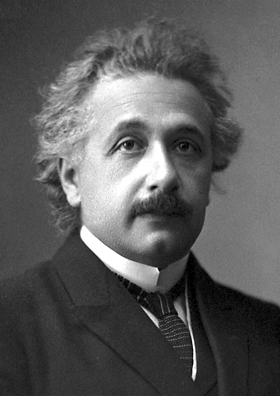
\includegraphics[height=5.4cm]{einstein_original_user.png}\\[-0.2em]
  \small（a）原图：皱纹、颗粒与局部明暗较明显
\end{minipage}
\hfill
\begin{minipage}[t]{0.43\textwidth}
  \centering
  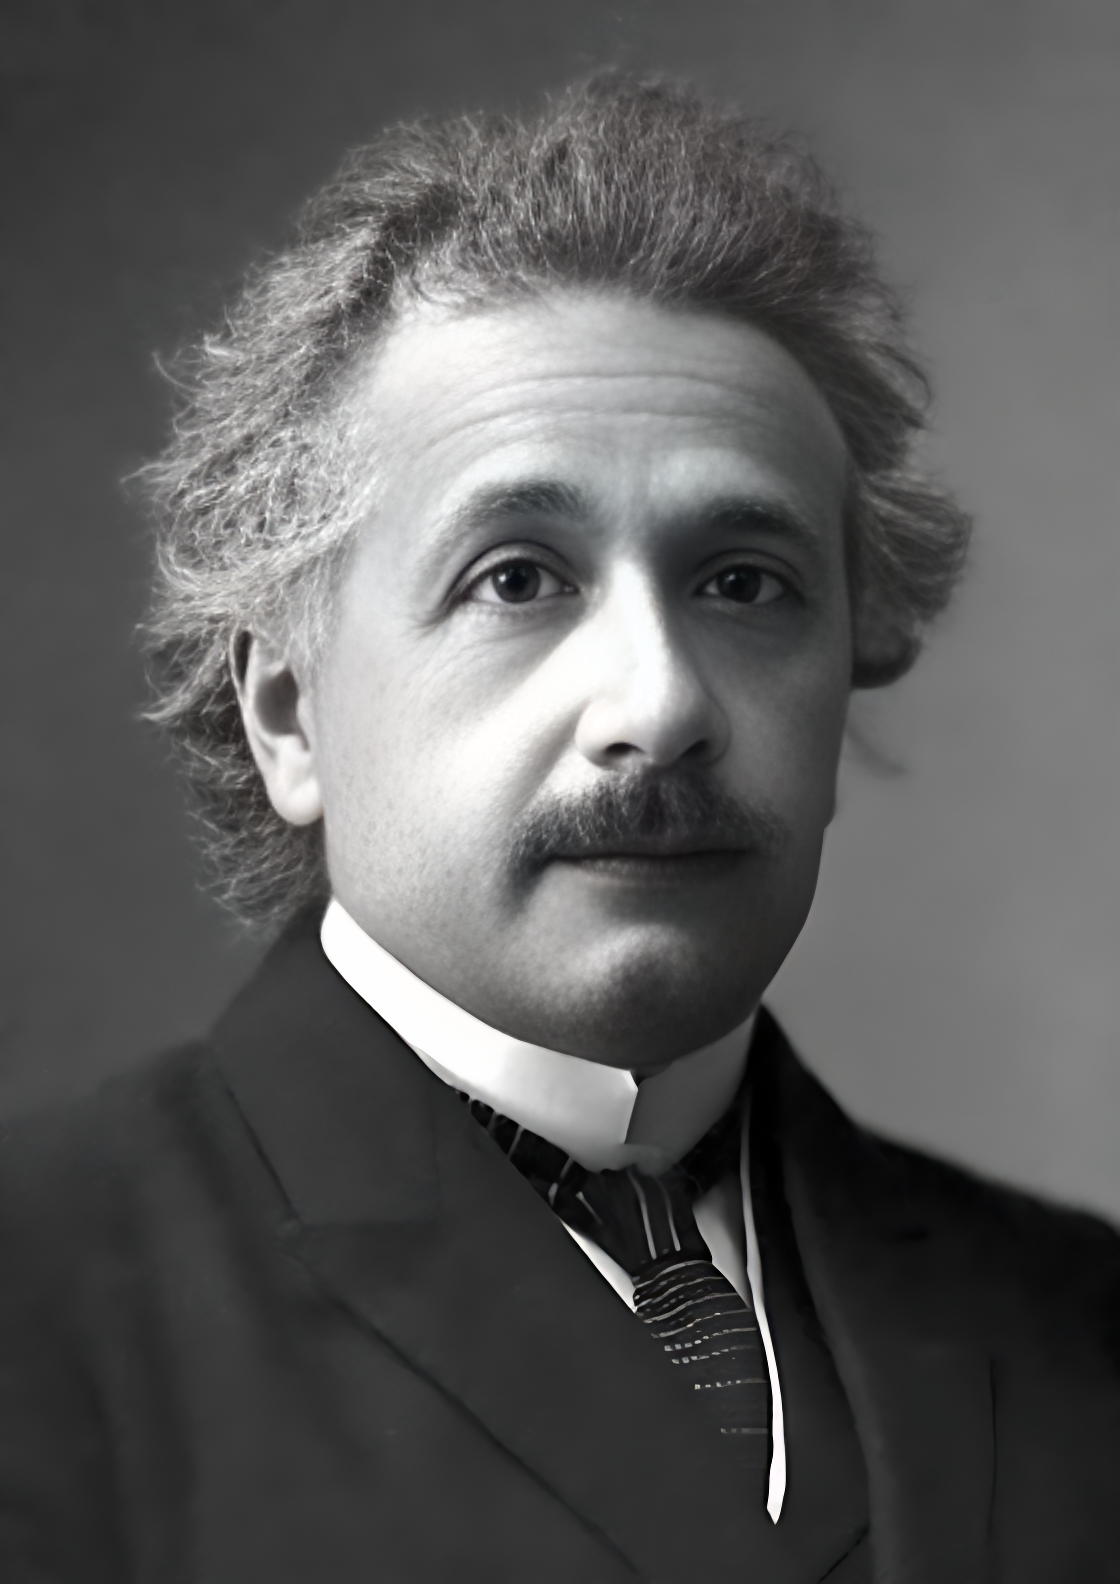
\includegraphics[height=5.4cm]{einstein_restored_user.png}\\[-0.2em]
  \small（b）GFPGAN：噪声减少，部分纹理被平滑或重绘
\end{minipage}
\caption{GFPGAN生成式修复同时带来去噪与纹理改写。图片来源：\href{https://replicate.com/tencentarc/gfpgan/examples\#2j4duq3vbfbblgd7jqx5xrcngi}{TencentARC/GFPGAN在线演示示例}（访问日期：2026-07-24）。}
\label{fig:einstein-demo}
\end{figure}

\paragraph{A/B1/C1实验。}
主分析只看冻结recoverable 40条Query。C1在该子组上直接复用B1，因此两者数值相同；C1的差别只体现在direct保留A、unusable拒绝。

\begin{table}[!htbp]
\centering
\caption{GFPGAN与缩放控制在recoverable组上的结果}
\label{tab:gfpgan-result}
\small
\begin{tabular}{lrrr}
\toprule
处理 & Rank-1 & 相对A & 救回/损害\\
\midrule
A原图 & \textbf{26/40（65.0\%）} & -- & --\\
B1 GFPGAN & 8/40（20.0\%） & $-45.0\pp$ & 0/18\\
C1 GFPGAN路由 & 8/40（20.0\%） & $-45.0\pp$ & 0/18\\
Resize512控制 & 26/40（65.0\%） & $0.0\pp$ & --\\
Resize-x2控制 & 26/40（65.0\%） & $0.0\pp$ & --\\
\bottomrule
\end{tabular}
\end{table}

表\ref{tab:gfpgan-result}给出本文主要结论：GFPGAN将recoverable组Rank-1由65.0\%降至20.0\%，下降45.0个百分点；B1与C1均没有救回任何原图错误样本，却损害18条原本正确样本。两种Resize控制保持65.0\%不变，说明下降不是由“放大后再压回112$\times$112”造成，而是来自模型对身份特征的改写。GFPGAN相对A的PID聚类置换检验$p=0.00125$。理论判断和实验结果指向同一结论：GFPGAN不适合作为当前身份识别链路的默认前处理。

\subsection{其他超分后端与场景适配性}

为判断问题是否只存在于GFPGAN，我们在同一冻结协议下加入CodeFormer\cite{codeformer}和Real-ESRGAN\cite{realesrgan}。CodeFormer使用$fidelity=1.0$；Real-ESRGAN只运行通用x2超分，不调用人脸增强模块。

\begin{table}[!htbp]
\centering
\caption{A/B1--3/C1--3主要结果}
\label{tab:multi-result}
\small
\begin{tabular}{lrrrr}
\toprule
后端 & Rank-1 & 相对A & 救回/损害 & B/C正确\\
\midrule
A原图 & \textbf{26/40} & -- & -- & --\\
GFPGAN & 8/40 & $-45.0\pp$ & 0/18 & 47/37\\
CodeFormer & 11/40 & $-37.5\pp$ & 0/15 & 58/40\\
Real-ESRGAN & 18/40 & $-20.0\pp$ & 1/9 & 74/47\\
\bottomrule
\end{tabular}
\par\vspace{0.2em}
\parbox{0.78\linewidth}{\raggedright\scriptsize 注：Rank-1为recoverable 40条；B/C正确数的分母均为156，C组拒绝82条unusable。}
\end{table}

三种超分的Rank-1都低于原图，Rank-5和MRR也保持相同排序。GFPGAN和CodeFormer只有损害、没有救回；PID聚类置换$p$分别为0.00125和0.00410。Real-ESRGAN救回1条、损害9条，点估计仍为负，但$p=0.31213$，不能声称存在稳定的人群级改善。

\begin{figure}[!htbp]
\centering
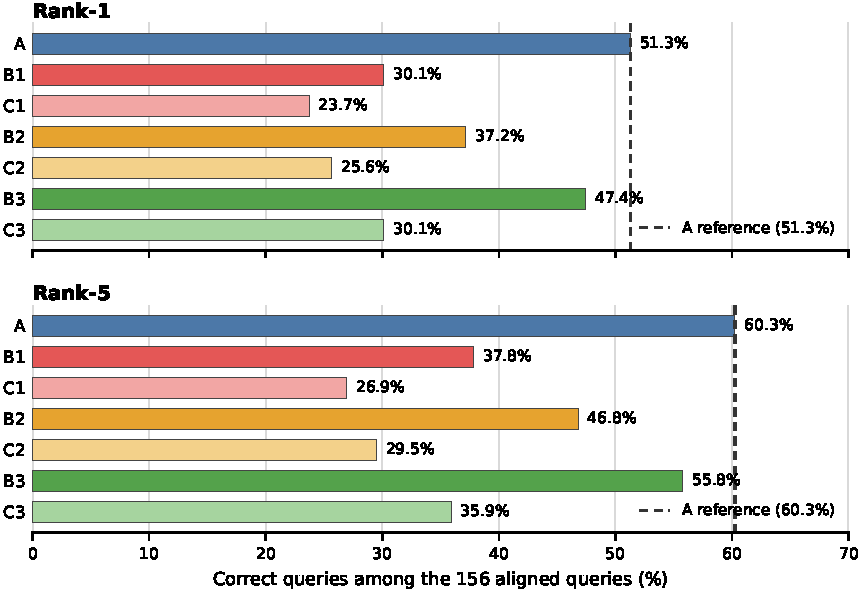
\includegraphics[width=0.72\textwidth]{all_aligned_rank1_rank5.pdf}
\caption{全部156条可对齐Query上的Rank-1（上）与Rank-5（下）。B1/C1、B2/C2、B3/C3分别对应GFPGAN、CodeFormer与Real-ESRGAN的全量处理和冻结路由；C组以156为共同分母，并将82条unusable拒绝计为未识别正确。虚线为各指标的A原图参考值。Rank-5仅表示真实身份进入前五候选，不等同于产品匹配成功。}
\label{fig:all-aligned-ranks}
\end{figure}

\begin{table}[!htbp]
\centering
\caption{156张可对齐Query上的速度与诊断结果}
\label{tab:backend-diagnostics}
\small
\begin{tabular}{lrrr}
\toprule
后端 & 秒/脸 & 原图--SR余弦 & FIQA变化\\
\midrule
GFPGAN & 0.236 & 0.402 & $+0.468$\\
CodeFormer & 0.324 & 0.584 & $+0.154$\\
Real-ESRGAN & \textbf{0.075} & \textbf{0.783} & $-0.142$\\
\bottomrule
\end{tabular}
\end{table}

Real-ESRGAN速度最快，与原图embedding也最接近，因此在三种方法中最适合做可选画面增强；但它仍比原图低20个百分点，不能替换身份识别输入。GFPGAN和CodeFormer虽然提高FIQA，却带来更大的身份漂移，再次说明FIQA不是身份保持指标。图\ref{fig:all-aligned-ranks}概括了全量结果：Rank-5在所有组中均高于Rank-1，说明保留候选集有利于后续再判定；但三种超分及对应路由在两个指标上均未超过A，整体排序也没有改变。

为避免与图\ref{fig:quality-samples}重复，图\ref{fig:qualitative-scores}改用三个新的身份与采集条件。direct样例满足B2/B3正确且达到0.45阈值、B1未达到阈值。冻结recoverable 40条中不存在B2/B3均达到阈值而B1未达到的样本，因此该行采用最接近的真实对照：B2/B3的Rank-1均正确、B1错误，但三种超分分数都低于阈值。第三行展示unusable边界，即使B3把真实身份排到第一，产品仍应按路由和阈值拒绝。这些定性样例只解释后端行为，不替代全量统计。

\begin{figure}[!htbp]
\centering
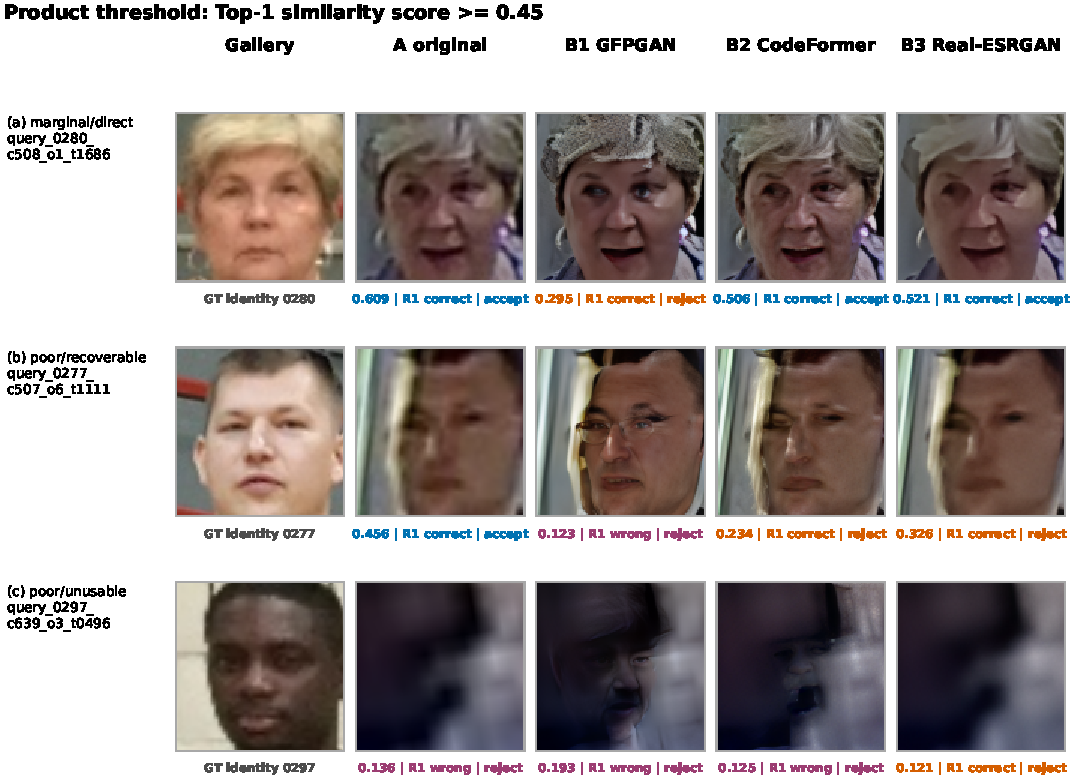
\includegraphics[width=0.99\textwidth]{qualitative_scores_grid.pdf}
\caption{三个未在图\ref{fig:quality-samples}出现的冻结Query在A原图与三种超分后端下的视觉和检索结果。每项标注真实Top-1相似度、Rank-1正确性与产品裁决；产品仅按Top-1相似度$\geq0.45$接受匹配。direct样例中B2/B3被接受而B1被拒绝；recoverable样例中B2/B3虽Rank-1正确但仍低于阈值；unusable样例仅B3 Rank-1正确，但路由与低分数均要求拒绝。}
\label{fig:qualitative-scores}
\end{figure}

\FloatBarrier
\section{结论}

质量分桶应由可解释的硬门槛和缺陷类型驱动。CR-FIQA只能作为诊断信号，不能证明处理前后身份不变，也不应改变direct、recoverable、unusable和none的成员。

从理论和实验两个角度看，GFPGAN不适合作为当前监控身份识别的默认前处理。扩展到CodeFormer和Real-ESRGAN后，三种超分的Rank-1和Rank-5仍都低于原图。Real-ESRGAN身份漂移最小、速度最快，但当前结果只支持把它用于人工查看或离线诊断。

这些结果对应的工程含义是：超分模块保持可插拔且默认关闭；身份链路继续使用原始对齐脸，超分输出仅用于人工查看或离线诊断，不自动写入Gallery，也不替换ArcFace输入。产品可以保留Top-5候选供多帧聚合或二次排序，但不能把“真实身份进入前五”直接视为匹配成功；最终命中仍应由独立校准后的Top-1分数阈值裁决，本实验沿用$\geq0.45$。

本实验的recoverable组只有40条Query，且缺少独立impostor Query；结论仅适用于当前MEVID、ArcFace和三个冻结后端。下一步应先改进人脸感知选帧、多帧特征聚合和原始采集质量，再在更多独立身份与真实客户回放上评估以身份保持为目标的超分方法。CodeFormer若进入产品评估，还需单独完成许可证审查。

\small
\begin{thebibliography}{9}
\setlength{\itemsep}{0.15em}

\bibitem{arcface}
J. Deng, J. Guo, N. Xue, and S. Zafeiriou,
``ArcFace: Additive Angular Margin Loss for Deep Face Recognition,''
\textit{Proceedings of the IEEE/CVF Conference on Computer Vision and Pattern Recognition},
2019.

\bibitem{gfpgan}
X. Wang, Y. Li, H. Zhang, and Y. Shan,
``Towards Real-World Blind Face Restoration with Generative Facial Prior,''
\textit{Proceedings of the IEEE/CVF Conference on Computer Vision and Pattern Recognition},
2021.

\bibitem{perceptiondistortion}
Y. Blau and T. Michaeli,
``The Perception-Distortion Tradeoff,''
\textit{Proceedings of the IEEE/CVF Conference on Computer Vision and Pattern Recognition},
2018.

\bibitem{pulse}
S. Menon, A. Damian, S. Hu, N. Ravi, and C. Rudin,
``PULSE: Self-Supervised Photo Upsampling via Latent Space Exploration of Generative Models,''
\textit{Proceedings of the IEEE/CVF Conference on Computer Vision and Pattern Recognition},
2020.

\bibitem{crfiqa}
F. Boutros, M. Fang, M. Klemt, B. Fu, and N. Damer,
``CR-FIQA: Face Image Quality Assessment by Learning Sample Relative Classifiability,''
\textit{Proceedings of the IEEE/CVF Conference on Computer Vision and Pattern Recognition},
2023.

\bibitem{codeformer}
S. Zhou, K. C. K. Chan, C. Li, and C. C. Loy,
``Towards Robust Blind Face Restoration with Codebook Lookup Transformer,''
\textit{Advances in Neural Information Processing Systems},
2022.

\bibitem{realesrgan}
X. Wang, L. Xie, C. Dong, and Y. Shan,
``Real-ESRGAN: Training Real-World Blind Super-Resolution with Pure Synthetic Data,''
\textit{Proceedings of the IEEE/CVF International Conference on Computer Vision Workshops},
2021.

\end{thebibliography}
\normalsize

\end{document}
